% !TEX root = ../main.tex
%Conclusie

\chapter{Conclusie.}
Door het analyseren van de gegeven vergelijkingen, vinden we twee evenwichten: 1: $(X_1, S_1) = (0, \alpha_2)$ en 2: $(X_2, S_2) = \left( \alpha_1\alpha_2 - \frac{1}{\alpha_1 - 1} - 1, \frac{1}{\alpha_1 - 1}\right)$. Uit niet door ons uitgevoerd onderzoek (zie bron 1) volgt dat er enkel realistische waarden $0.7< \alpha_1 < 2.4$ bestaan. Uit de vergelijkingen volgt direct dat als $\alpha_1 \leq 1$, dan hebben we te maken met een daling van de bacterie populatie en komen we uiteindelijk bij het triviale evenwicht uit. 

Door verdere analyse uit te voeren, vinden we dat evenwicht 1 stabiel is als $\alpha_2 < \frac{1}{\alpha_1 - 1}$ (en het triviale evenwicht), zo niet dan hebben we te maken met een zadelpunt. Voor evenwicht twee gelden dezelfde voorwaarden. Voor beide resultaten, lees hoofdstuk 5. 

Een voorbeeld van een stabiel evenwicht is dus $\alpha_1 = 1.30$ en $\alpha_2 = 4.2 (> \frac{1}{\alpha_1 - 1})$. De bijbehorende grafiek (gevonden door gebruik te maken van de methode van Euler (zie hoofdstuk 4)), met beginwaarden $S(0) = 0.5$ en $X(0) = 0.4$

\begin{figure}[h]
	\centering
	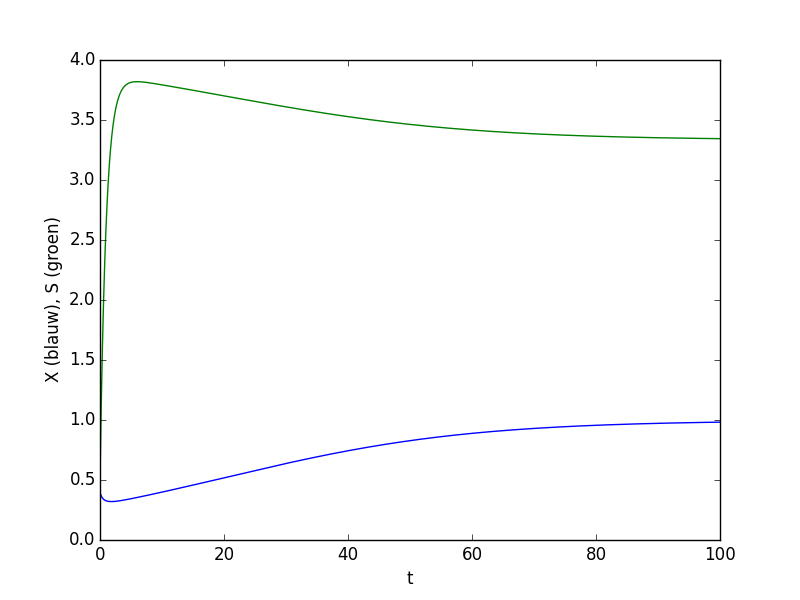
\includegraphics[width=0.6\textwidth]{../images/figure_5.png}
	\caption{Bacterie- en voedselconcentratie tegen elkaar.}
\end{figure}

We zien dus dat het erg zal afhangen van de kosten en de precieze doelen van de reactor, wat de precieze beginwaarden zullen moeten zijn. Als het immers erg belangrijk is dat een evenwicht zich snel vestigt, moeten natuurlijk $S(0)$ en $X(0)$ zo gekozen worden dat ze in de buurt van de evenwichtswaarden liggen. 